\begin{figure}[h]
    \centering
    \captionsetup{width=.9\linewidth}
    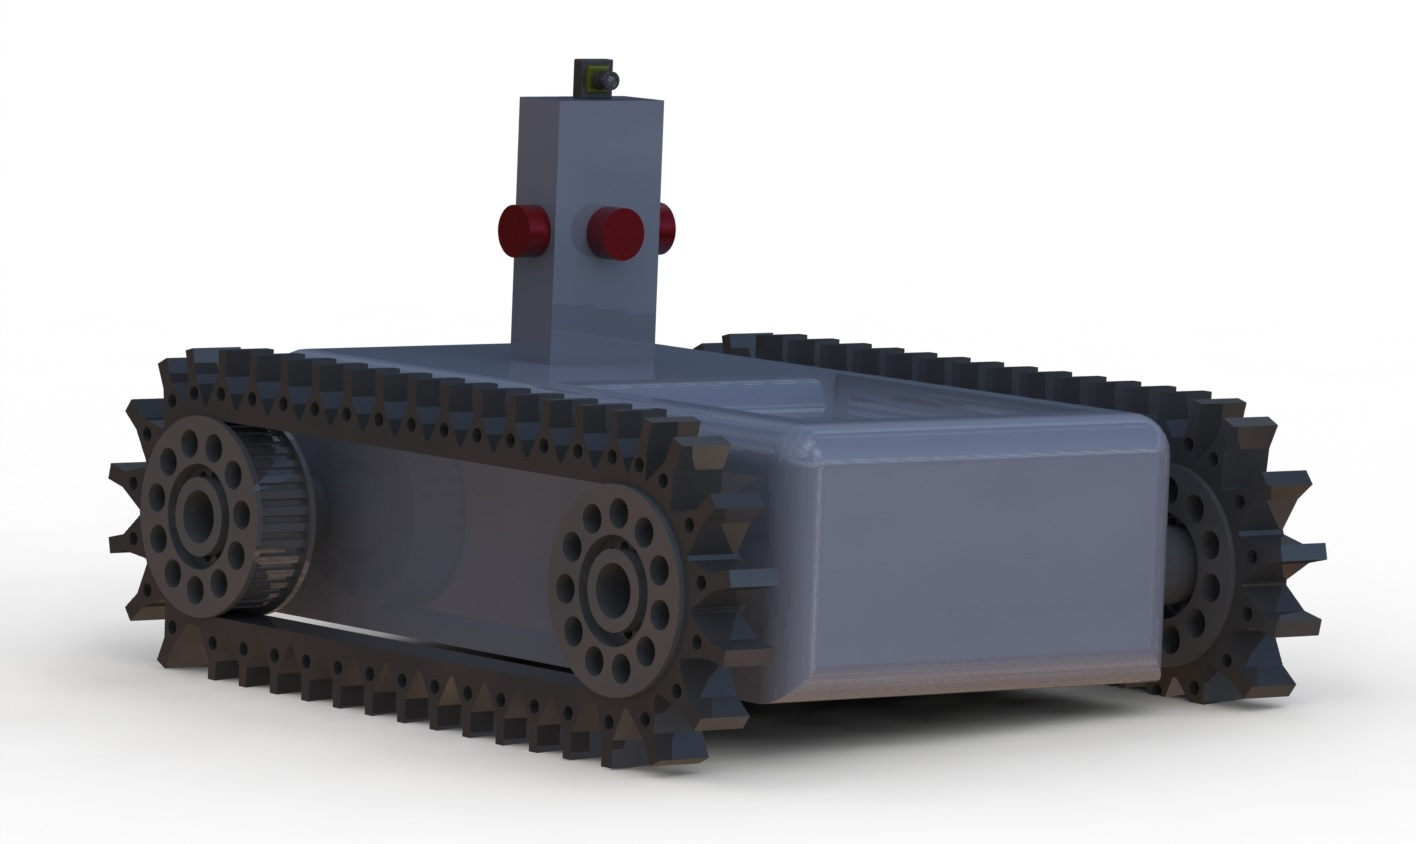
\includegraphics[width=1\linewidth]{v2_rendering.JPG}
    \caption{Erster Prototyp}
    \label{fig:prot}
\end{figure}

Das 3D-Modell des Rettungsroboters wurde mit der Software SolidWorks erstellt. Die Abbildung \ref{fig:prot} zeigt den ersten Prototyp. Hier wurden schon der Kettenantrieb und eine Ablagefläche für ein Erste-Hilfe-Kit umgesetzt. Weiter wurde auf dem Robotor ein Turm platziert, um dort 4 Sensroen für die Orientierung anzubringen. Oben auf dem Turm befindet sich eine Kamera.\\


\begin{figure}[h]
    \centering
    \captionsetup{width=.9\linewidth}
    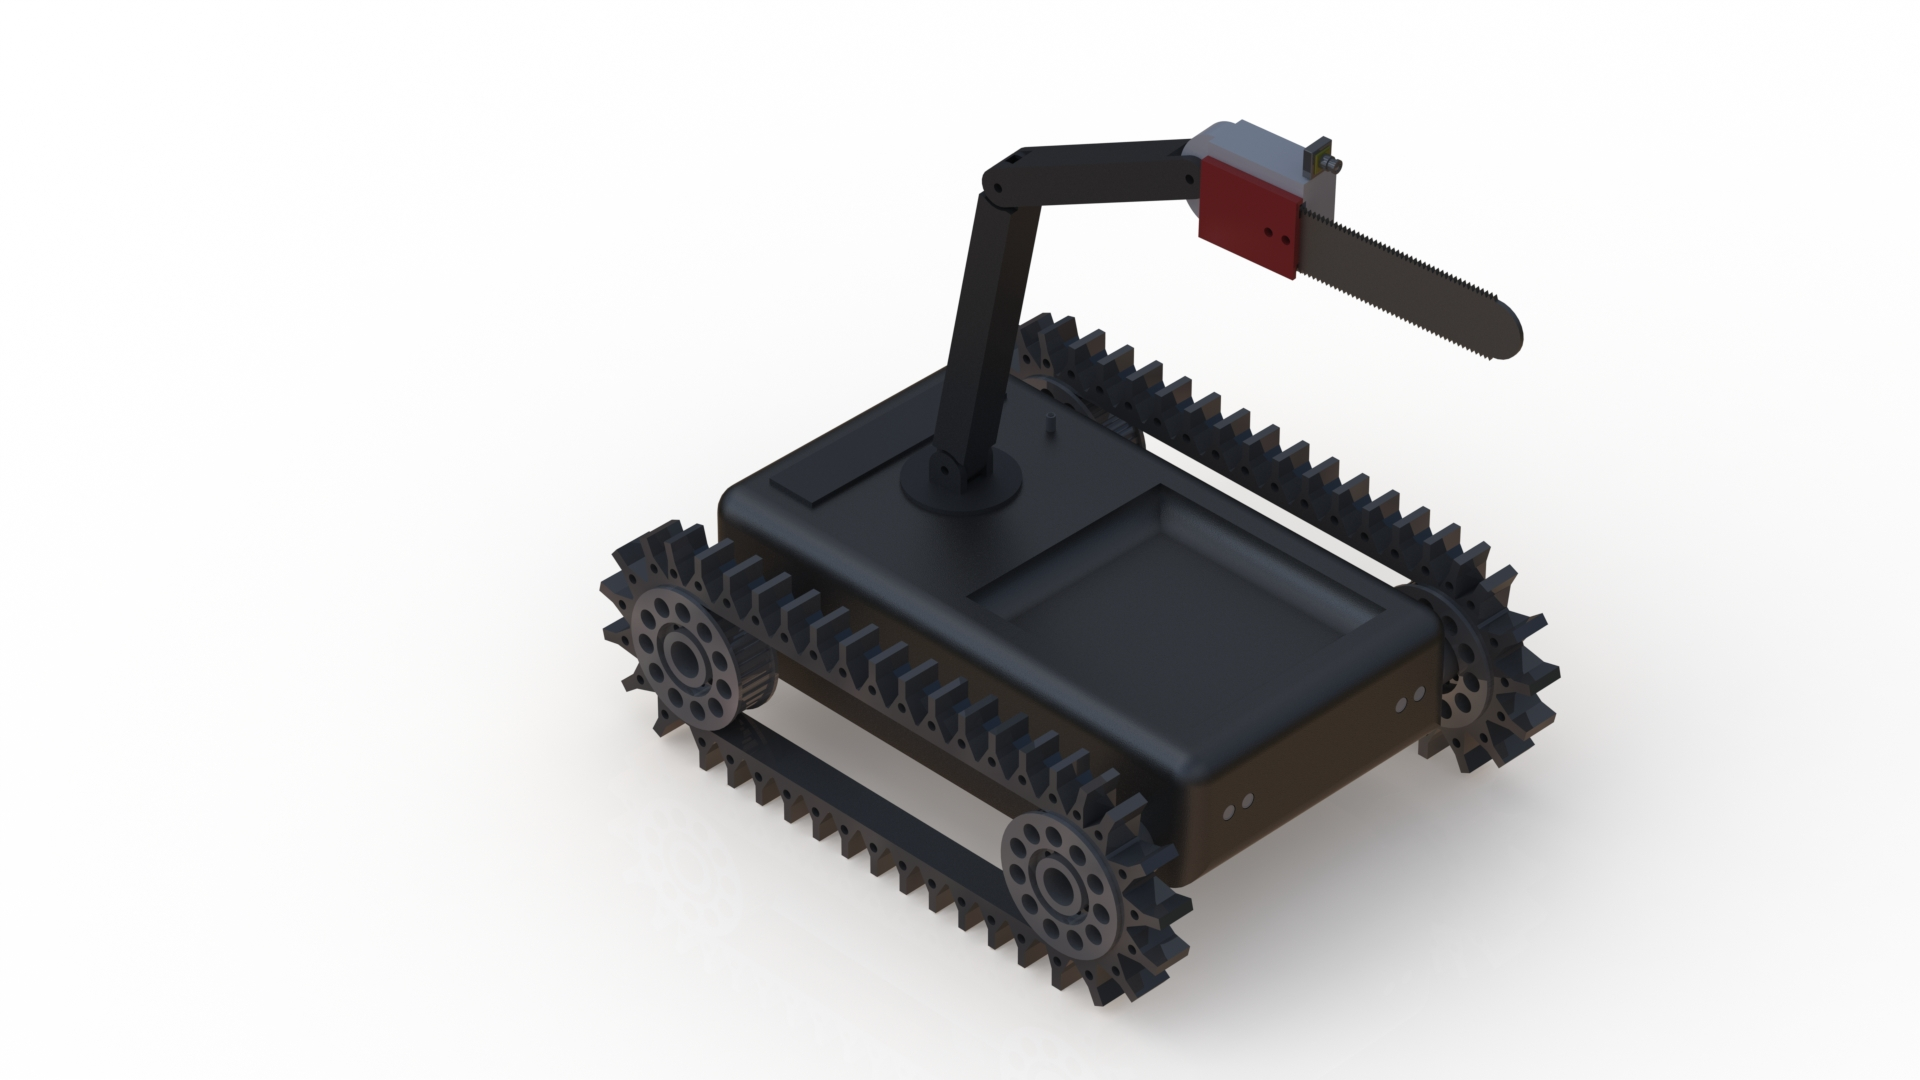
\includegraphics[width=1\linewidth]{bot_rendering_v4.JPG}
    \caption{Zweite Version den Roboters}
    \label{fig:second}
\end{figure}

Für die zweite Version des Prototyps wurde zunächst der Körper des Bots angepasst. Für eine Verbesserung des Strömungsverhaltens und einer Erhöhung des Böschungswinkels wurde der Körper an der vorderen unteren Kante mit einer sehr Flachen Fase versehen.

Im nächsten Schritt wurde der unbewegliche Turm durch einen Roboterarm mit 3 Gelenken und einer Drehscheibe ersetzt (Abb. \ref{fig:second}). Am Ende des Arms wurde eine Kettensäge angebracht. Die Kamera wurde auf der Säge angebracht, um so die Säge immer im Blick zu haben.

Weiter wurden noch ein austauschbarer Akku, ein omnidirektionales Mikrofon und Ultraschallsensoren in den Prototyp intgeriert.
\begin{figure}[h]
    \centering
    \captionsetup{width=.9\linewidth}
    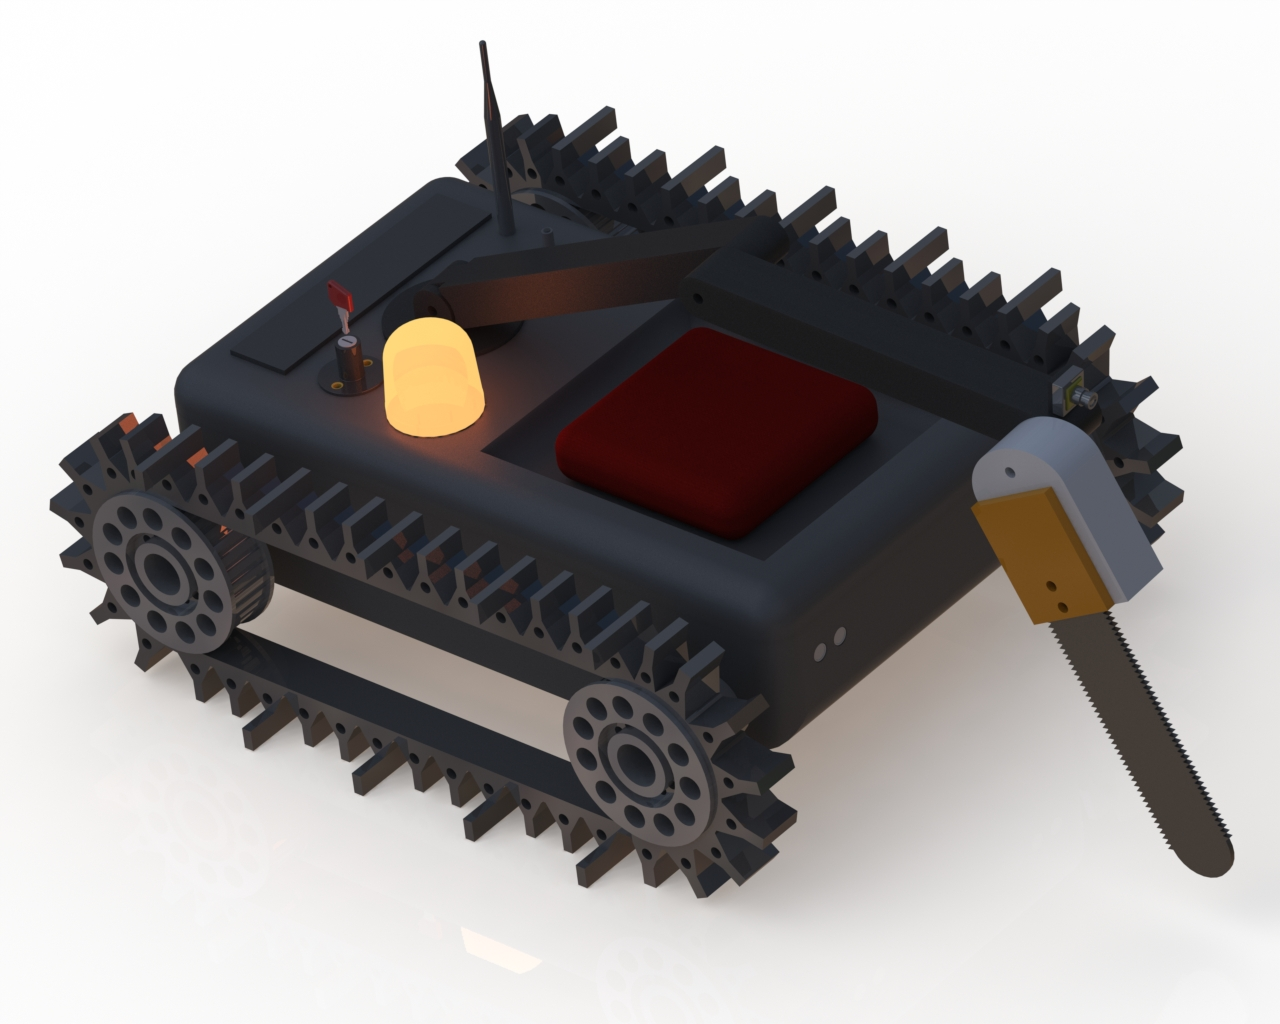
\includegraphics[width=1\linewidth]{trimetrisch_vorne_rechts_oben.JPG}
    \caption{Außenansicht des Roboters}
    \label{fig:final}
\end{figure}
\begin{figure}[h]
    \centering
    \captionsetup{width=.9\linewidth}
    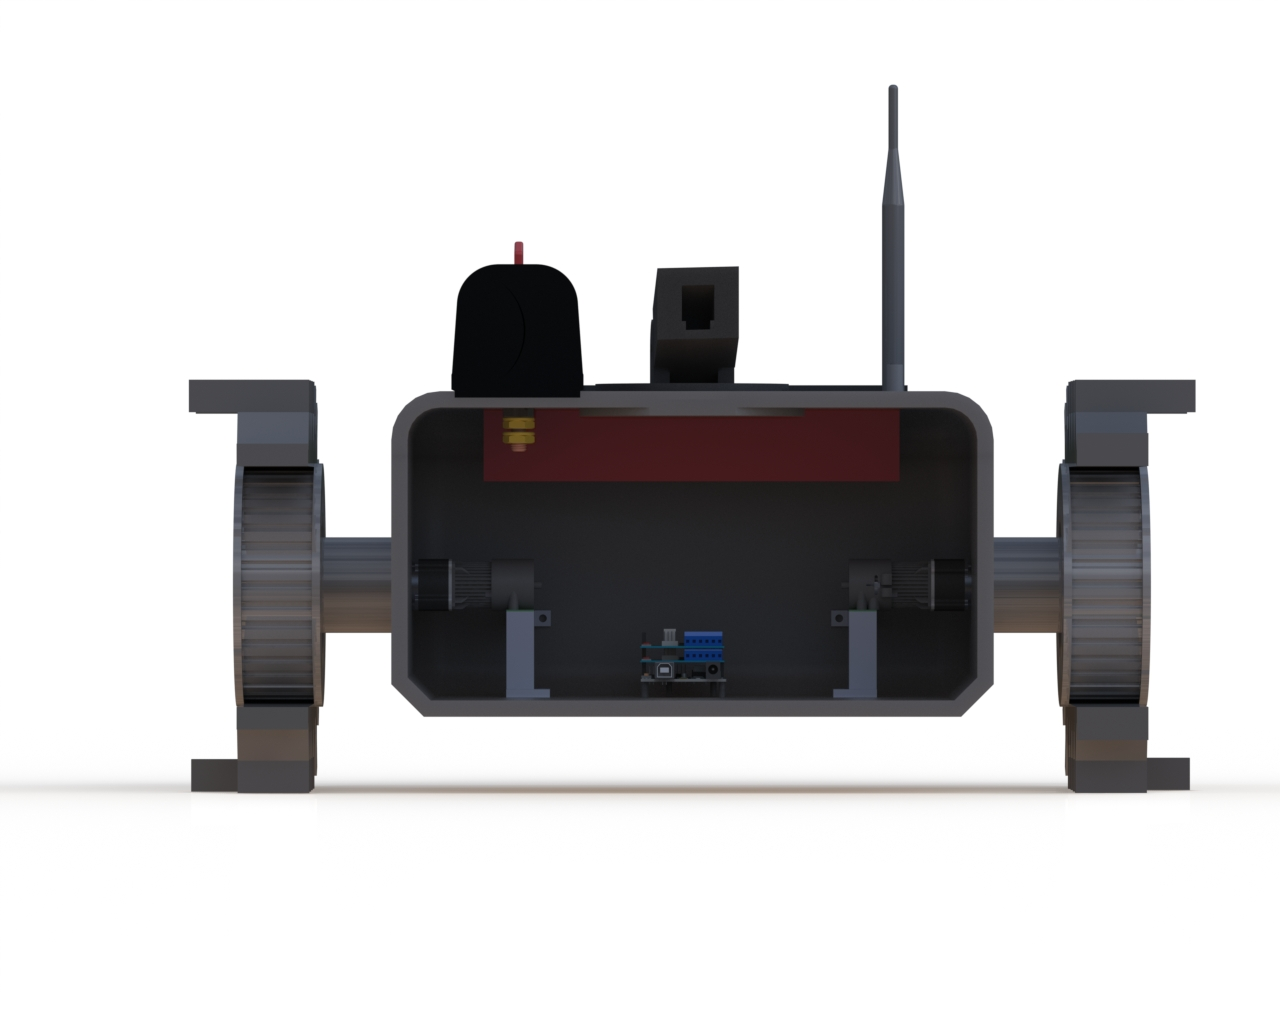
\includegraphics[width=1\linewidth]{schnitt_front.JPG}
    \caption{Schnittansicht von vorne}
    \label{fig:front}
\end{figure}
\begin{figure}[h]
    \centering
    \captionsetup{width=.9\linewidth}
    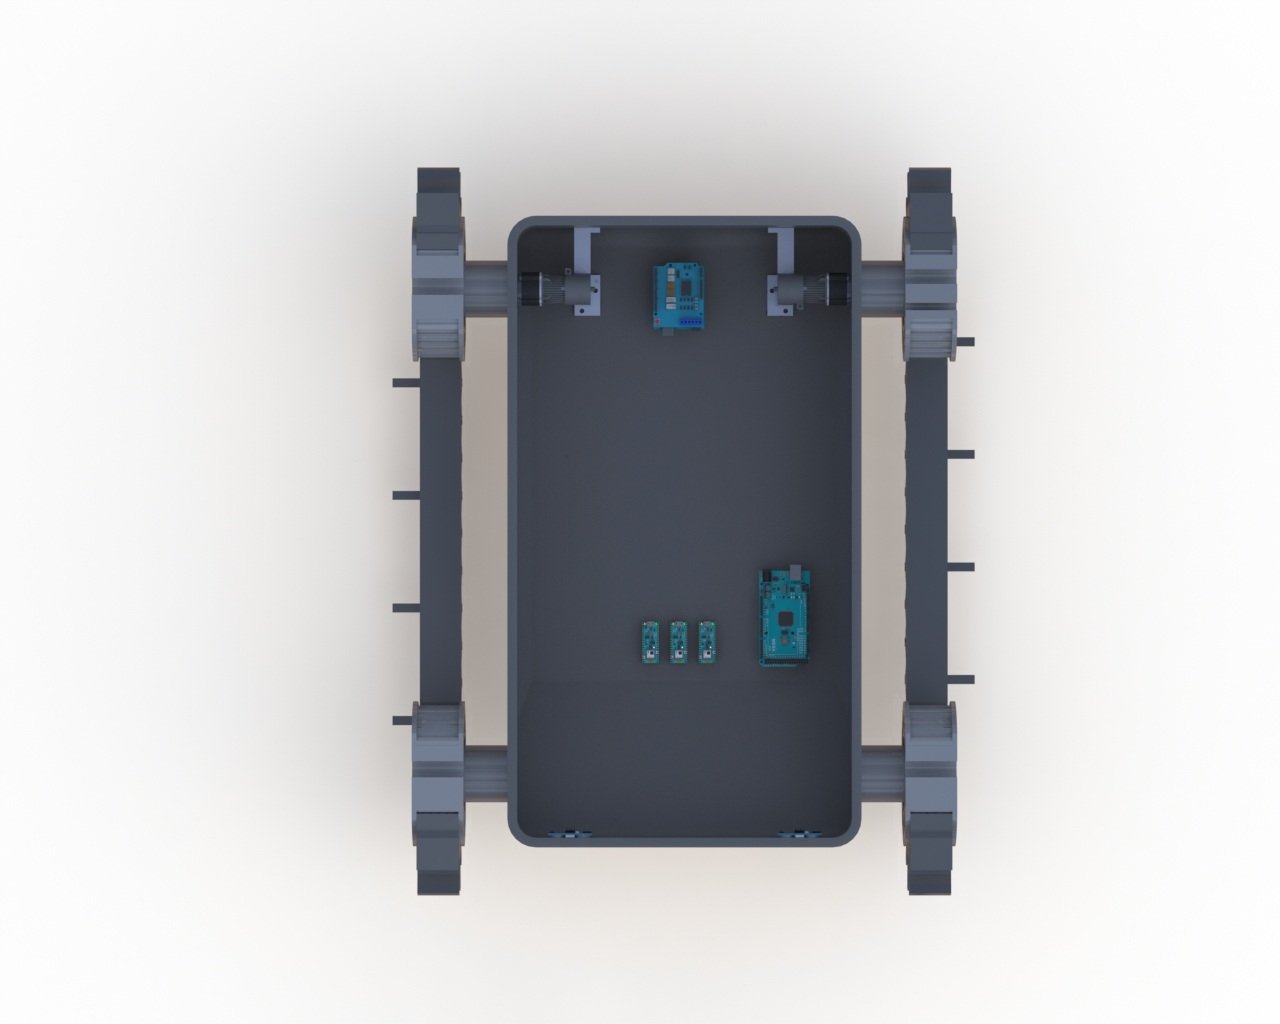
\includegraphics[width=1\linewidth]{schnitt_top.JPG}
    \caption{Schnittansicht von oben}
    \label{fig:top}
\end{figure}
\begin{figure}[h]
    \centering
    \captionsetup{width=.9\linewidth}
    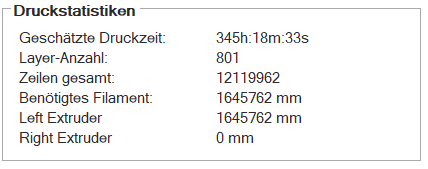
\includegraphics[width=1\linewidth]{print-statistic.PNG}
    \caption{Druckstatistiken}
    \label{fig:print_stats}
\end{figure}
\begin{figure}[h]
    \centering
    \captionsetup{width=.9\linewidth}
    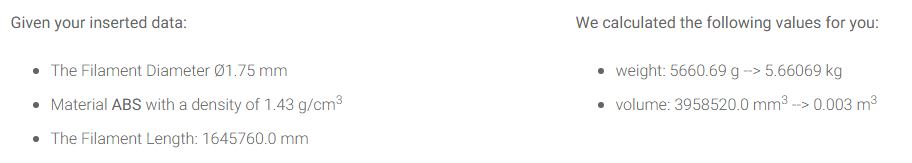
\includegraphics[width=1\linewidth]{filament_weight.PNG}
    \caption{Erechnetes Filamentgewicht}
    \label{fig:filament_weight}
\end{figure}